\chapter{Random Number Generators}
Random Numbers are used in a variety of applications, for example:
\begin{itemize}
  \item simulating random events
  \item professional gaming
  \item end-of-production & in-field testing of digital systems
  \item Monte Carlo algorithms
  \item cryptographic applications
\end{itemize}
A random number can be generated both via software, or via hardware.\\
Random number are usually needed to generate, in cryptography, some secret data, that is not known 
and unpredictable to an authorized user. To achieve this, the randomization is uslaly employed.\\

\begin{boxH}
  A Random Number Generator (RNG) is a utility or device that produces a sequence of numbers 
  within an interval [min, max] while guaranteeing that values appear unpredictable.
\end{boxH}

\begin{subsection}{Characteristics of Random Number generators}
  An RNG should have the following \textbf{3 characteristics}:
  \begin{itemize}
    \item Each new value must be \textbf{statistically independent} of the \textbf{previous value}.
      \subitem That is, given a generated sequence of values, a particular value is not more likely 
       to follow it as the next value in the RNG's random sequence.
    \item The overall distribution of numbers chosen from the interval is \textbf{uniformly distributed}.
      \subitem In other words, all numbers are equally likely, and no one is more “popular” or 
        appears more frequently in the RNG’s output than others.
    \item The sequence is \textbf{unpredictable}
      \subitem An attacker cannot guess some or all the values in a generated sequence. Predictability 
        may take the form of forward prediction (future values) and backtracking (past values).
  \end{itemize}

  In general, the lack of even one of those qualities can intoduce severe security vulnerabilities
  that can be exploited by an attacker.\\
  For this reason, the level of care required during the design and implementation of an RNG is
  at leas the same requeired for any other element of a cryptographic system.
\end{subsection}
\begin{paragraph}{Attack on random numbers}
  Back in the days, some attacks were possible on RNGs, for example the netscape implementation of 
  SSL used a RNG that was predictable, or in Java, it was possible to predict the session ids.\\
  those attacks were possible because the random numbers generated wer not unpredictable, being very 
  weak, making it possible to an attackers to break the system.\\
\end{paragraph}
\begin{section}{True Random Number generators}
  \begin{boxH}
    A True Random Number Generator (TRNG) is a device that generates random numbers from a physical 
    process, rather than a deterministic algorithm, removing all the entropy from the physical world.
  \end{boxH}
  TRNGs are thus often called non-deterministic random number generators since the next number to 
  be generated cannot be determined in advance.\\
  The physical process can be any process that is unpredictable, such as:
  \begin{itemize}
    \item radioactive decay
    \item thermal noise(Johnson-Nyquist noise, or resistor noise)
    \item avalanche noise
    \item timing of keystrokes
    \item audio
  \end{itemize}
  The generated numbers are truly random, and are not predictable by any algorithm.\\
  The main problem with TRNGs is that they are slow, and they are not suitable for all applications.
  \begin{paragraph}{The most common Analog source}
    The most adopted solutions rely on the following:
    \begin{itemize}
      \item amplifying the noise generated by a resistor (Johnson noise) or by a semiconductor diode
      \item feeding the noise to a comparator or Schmitt trigger
      \item sampling the output of the comparator to get a series of bits that can be used to
        generate random numbers.
    \end{itemize}
  \end{paragraph}
  In some applications, TRNG is implemented simply by measuring internal computer activities that are quantifiable and genuinely random without
  resorting to external custom analog devices.
  \begin{figure}
    \centering
    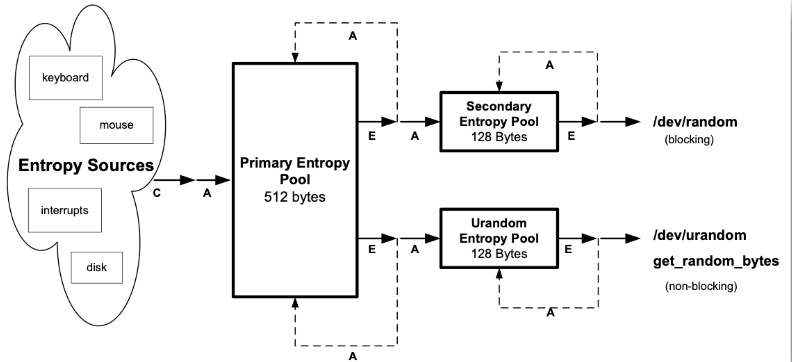
\includegraphics[width=0.5\textwidth]{img/hardware/linux rng.png}
    \caption{the TRNG in the Linux kernel}
  \end{figure}
  To wrap this section up, using system clock, process scheduling, and other system effects may 
  result in some values occurring far more frequently than others:
  \begin{itemize}
    \item When dealing with human-generated entropy, values do not distribute evenly across
      the space of all possible values: some values are more likely to occur than others, and 
      certain values rarely occur in practice.
    \item The entropy in the operating system is usually limited, and waiting for more entropy is
      slow and impractical
\end{section}
\begin{section}{Pseudo-Random number generators}
  \begin{boxH}
    A PRNG is an algorithm or a hardware device that generates a sequence of random bits 
    (or numbers), starting from an initial value called the seed.
  \end{boxH}
  the most common exaple of this class of RNG is the rand() function in the C standard 
  library.\\
  PNRGS have a characteristic that can be a issue if not properly handled: numbers \textbf{repets periodically}
  and this periodicity depends on the size of the internal state model of the PRNG.
  This is not always a issue for not security related purposes, but mostly this Characteristic can 
  be a dealbreaker for many applications.\\
  The best PRNG algorithms available today have such a large period that this weakness can be 
  practically ignored. For example, the Mersenne Twister MT19937 PRNG with 32-bit word length has a
  periodicity of 219937-1.\\
  Nevertheless, perfect knowledge of the generating circuit and the most
  recently generated numbers could enable one to guess the next number to
  be generated. For this reason, w test the values to know how longer we can stick to 
  th generated sequence before updating it.
  \begin{boxH}
    While a generated sequence of values exhibits the statistical properties
    of randomness (independence, uniform distribution), the overall behaviour of
    the PRNG is entirely predictable.
  \end{boxH}
  For this reason, PRNGs are often called Deterministic random number generators since, given a 
  particular seed value, the same PRNG will always produce the same sequence of “random” numbers.
  \begin{subsection}{Seed criticality}
    To ensure forward unpredictability, care must be taken when obtaining seeds, which should be a 
    true random number.
    After all, the values produced by a PRNG are completely predictable if both the seed and the
    generation algorithm are known.
    Since, in many cases, the generation algorithm is publicly available, the seed
    must be kept secret and generated from a TRNG.

  \end{subsection}

\end{section}

